\documentclass[12pt, a4 paper]{article}
% Set target color model to RGB
\usepackage[inner=2.0cm,outer=2.0cm,top=2.5cm,bottom=2.5cm]{geometry}
\usepackage{setspace}
\usepackage[rgb]{xcolor}
\usepackage{environ}
\usepackage{verbatim}
\usepackage{subcaption}
\usepackage{outlines}
\usepackage{amsgen,amsmath,amstext,amsbsy,amsopn,tikz,amssymb,tkz-linknodes}
\usepackage{fancyhdr}
\usepackage{pgfplots}
\usepackage{mathtools}
\usepackage{graphicx}
\usepackage[colorlinks=true, urlcolor=blue,  linkcolor=blue, citecolor=blue]{hyperref}
\usepackage[colorinlistoftodos]{todonotes}
\usepackage{rotating}
\usepackage{enumitem}

\linespread{1.6} % Double Line Spacing

\usetikzlibrary{arrows.meta,intersections,calc}
\graphicspath{ {./img/} }

\hypersetup{%
pdfauthor={Vignesh Ravibaskar},%
pdfcreator={PDFLaTeX},%
pdfproducer={PDFLaTeX},%
}

\setlist[enumerate,1]{label=\textbf{\arabic*}}
\setlist[enumerate,2]{label=\textbf{({\alph*})}}
\setlist[enumerate,3]{label=\textbf{({\roman*})}}

\title{Integration}
\author{Derek, Vignesh}
\date{2020}

\newcommand{\comm}[1]{}
\NewEnviron{answer}{\vspace{3mm} \\ \color{blue} {\BODY} \color{black}}
% \NewEnviron{answer}{\color{blue} \comm{\BODY} \color{black}} % Use this method to hide all answers

\begin{document}

\maketitle

\textbf{INTEGRATION [80 Marks]}
\begin{outline}[enumerate]
	\1 Integrate the following:
	\2 $\int \tan^{-1}(\dfrac{\pi}{3}x)\,\mathrm{d}x$\hfill[4]
	\begin{answer}
		Integrating by Parts:
		\begin{align*}
			\int \tan^{-1}(\frac{\pi}{3}x)\,\mathrm{d}x
			  & = x\tan^{-1}(\frac{\pi}{3}x)-\int\frac{\pi/3\cdot x}{1+\pi^2/9\cdot x^2}\,\mathrm{d}x \\&= x\tan^{-1}(\frac{\pi}{3}x)-\int \frac{3\pi x}{\pi^2x^2+9}\,\mathrm{d}x \\
			  & = x\tan^{-1}(\frac{\pi}{3}x) - \frac{3}{2\pi}\ln{|\pi^2x^2+9|} + C
		\end{align*}
	\end{answer}
	\2 $\int x^3\mathrm{e}^{3x} \,\mathrm{d}x$\hfill[4]
	\begin{answer}
		Integrating by Parts Repeatedly:
		\begin{align*}
			\int x^3\mathrm{e}^{3x} \,\mathrm{d}x & = \frac{1}{3}x^3\mathrm{e}^{3x}-\int x^2\mathrm{e}^{3x}\,\mathrm{d}x                                                          \\&=\frac{1}{3}x^3\mathrm{e}^{3x} - \frac{1}{3}x^2\mathrm{e}^{3x}+\frac{2}{3}\int x\mathrm{e}^{3x}\,\mathrm{d}x \\
			                                      & = \frac{1}{3}x^3\mathrm{e}^{3x} - \frac{1}{3}x^2\mathrm{e}^{3x} - \frac{2}{9}x\mathrm{e}^{3x} - \frac{2}{27}\mathrm{e}^{3x}+C
		\end{align*}
	\end{answer}
	\2 $\int_{-\frac{1}{2}}^1 \frac{1}{\sqrt{(1-x)(x+2)}}\,\mathrm{d}x$\hfill[4]
	\begin{answer}
		Completing the Square and then Integrating:
		\begin{align*}
			\int_{-\frac{1}{2}}^1 \frac{1}{\sqrt{(1-x)(x+2)}}\,\mathrm{d}x & = \int_{-\frac{1}{2}}^1 \frac{1}{\sqrt{-x^2-x+2}}\,\mathrm{d}x    \\&= \int_{-\frac{1}{2}}^1 \frac{1}{\sqrt{(\frac{3}{2})^2-(x+\frac{1}{2})^2}}\,\mathrm{d}x \\
			                                                               & = [\sin^{-1}{\frac{x+\frac{1}{2}}{\frac{3}{2}}}]_{-\frac{1}{2}}^1 \\
			                                                               & = \sin^{-1}1-\sin^{-1}0 = \frac{\pi}{2}
		\end{align*}
	\end{answer}
	\2 $\int_0^{\ln2} \dfrac{1}{e^x+e^{2x}}\,\mathrm{d}x$, using the substitution $x = \ln u$. \hfill[5]
	\begin{answer}
		Substituting $x=\ln u$ and $\,\mathrm{d}x = \dfrac{1}{u} \,du$:
		\begin{equation*}
			\int_0^{\ln2} \frac{1}{e^x+e^{2x}}\,\mathrm{d}x = \int_1^2 \frac{1}{u^2(u+1)}\,du
		\end{equation*}
		Using the Partial Fraction Decomposition:
		\begin{equation*}
			\frac{1}{u^2(u+1)} = \frac{A}{u} + \frac{B}{u^2} + \frac{C}{u+1} \quad \textrm{where} \quad A,B,C\in\mathbb{Q}
		\end{equation*}
		We can use the Cover-Up Method to get B and C:
		\begin{equation*}
			B = \frac{1}{0+1}=1, \quad C = \frac{1}{(-1)^2} = 1
		\end{equation*}
		Multiplying both sides by $u^2(u+1)$:
		\begin{equation*}
			1 = Au(u+1) + (u+1) + u^2
		\end{equation*}
		By Comparing the $x^2$ coefficient, it is evident that $A=-1$ Thus, our integration simplifies to:
		\begin{align*}
			\int_0^{\ln2} \frac{1}{e^x+e^{2x}}\,\mathrm{d}x & = \int_1^2 \frac{1}{u^2(u+1)}\,\mathrm{d}u =\int_1^2 -\frac{1}{u} + \frac{1}{u^2} + \frac{1}{u+1} \,\mathrm{d}u \\
			                                                & = [-\ln{|u|}-\frac{1}{u}+\ln{|u+1|}]_1^2 = \frac{1}{2}-2\ln{2}+\ln{3}
		\end{align*}
	\end{answer}
	\1 Show that ${\frac{\mathrm{d}}{\mathrm{d}x}}\cot{x}= -\csc^2x$.\\
	\begin{answer}
		Using the Fraction Rule:
		\begin{align*}
			{\frac{\mathrm{d}}{\mathrm{d}x}}\cot{x} = {\frac{\mathrm{d}}{\mathrm{d}x}}(\frac{\cos x}{\sin x}) & = \frac{-\sin x \times \sin x - \cos x \times \cos x}{\sin^2 x}          \\
			                                                                                                  & = -\frac{\sin^2 x + \cos^2 x}{\sin^2 x} = -\frac{1}{\sin^2 x} = -\csc^2x
		\end{align*}
	\end{answer}
	Hence or otherwise, find $\int \csc^3x\,\mathrm{d}x$, given that $0<x<\pi$. \hfill[6]
	\begin{answer}
		Integrating by Parts, then using the Pythagorean Identity $\cot^2 x+1=\csc^2 x$:
		\begin{align*}
			\int \csc^3x\,\mathrm{d}x & = -\csc x \cot x - \int \csc x \cot^2 x \,\mathrm{d}x                   \\
			                          & = -\csc x \cot x - \int \csc x (\csc^2 x -1) \,\mathrm{d}x              \\
			                          & = -\csc x \cot x + \int \csc x\,\mathrm{d}x - \int \csc^3x\,\mathrm{d}x \\
			                          & = -\csc x \cot x - \ln{|\csc x + \cot x|} - \int \csc^3x\,\mathrm{d}x
		\end{align*}
		Grouping $\int \csc^3x\,\mathrm{d}x$ on the LHS,
		\begin{align*}
			2\int \csc^3x\,\mathrm{d}x = -\csc x \cot x - \ln{|\csc x + \cot x|} + C             \\
			\int \csc^3x\,\mathrm{d}x = -\frac{1}{2}(\csc x \cot x + \ln{|\csc x + \cot x|}) + C
		\end{align*}
	\end{answer}
	\1 Show that $\cos{a\theta} \cos{3a\theta} = \dfrac{\cos{2a\theta} + \cos{4a\theta}}{2}$.\\
	\begin{answer}
		Using the identity $\cos p+\cos q=2\cos {\dfrac {p+q}{2}}\cos {\dfrac {p-q}{2}}$:
		\begin{align*}
			\cos{a\theta} \cos{3a\theta} & = \frac{\cos{2a\theta} + \cos{4a\theta}}{2}                                                  \\
			                             & = \frac{1}{2} \times (2 \cos{\frac{4a\theta-2a\theta}{2}} \cos{\frac{4a\theta+2a\theta}{2}}) \\
			                             & = \frac{\cos{2a\theta} + \cos{4a\theta}}{2}
		\end{align*}
	\end{answer}
	Hence by Integration by Parts, find $\int_0^{\pi/4} 2\theta\cos\theta\cos{3\theta}\,d\theta$. \hfill[6]
	\begin{answer}
		Using the above result:
		\begin{align*}
			\int_0^{\pi/4} 2\theta\cos\theta\cos{3\theta}\,\mathrm{d}\theta & = \int_0^{\pi/4} \theta(\cos{2\theta} + \cos{4\theta})\,\mathrm{d}\theta                                                                                       \\
			                                                                & = [\theta(\frac{1}{2}\sin{2\theta} + \frac{1}{4}\sin{4\theta})]_0^{\pi/4}-\int_0^{\pi/4} \frac{1}{2}\sin{2\theta} + \frac{1}{4}\sin{4\theta}\,\mathrm{d}\theta \\
			                                                                & =[\theta(\frac{1}{2}\sin{2\theta} + \frac{1}{4}\sin{4\theta}) + \frac{1}{4}\cos{2\theta} + \frac{1}{16}\cos{4\theta}]_0^{\pi/4}                                \\
			                                                                & = [\frac{\pi}{4}(\frac{1}{2}\sin{\frac{\pi}{2}})+ \frac{1}{16}\cos{\pi}]- (\frac{1}{4}+\frac{1}{16})                                                           \\
			                                                                & = \frac{\pi-3}{8}
		\end{align*}
	\end{answer}

	\1 A geometric progression has first term $a$ and common ration $x$, where $a,x \in \mathbb{R}$. The sum of the first $n$ terms of the geometric progression is denoted by $S_n$.
	\2 State in terms of $a$ and $x$, the $n$th term of the geometric progression.\hfill[1]
	\begin{answer}
		By the definition of a Geometric Progression, the $n$th term is $ax^{n-1}$
	\end{answer}
	\2 Given that the sum of the first $n$ terms of the Harmonic Series $1+\dfrac{1}{2}+\dfrac{1}{3}+\dots+\dfrac{1}{n}=H_n$, show that $\int_0^1 S_n\,\mathrm{d}x=aH_n$ \hfill[3]
	\begin{answer}
		Using the fact that $S_n = a\dfrac{x^n-1}{x-1}$:
		\begin{align*}
			\int_0^1 S_n\,\mathrm{d}x = \int_0^1 a\frac{x^n-1}{x-1}\,\mathrm{d}x & = a\int_0^1 x^{n-1}+x^{n-2}+x^{n-3}+\dots+x^2+x+1\,\mathrm{d}x                                     \\
			                                                                     & = a[\frac{x^n}{n}+\frac{x^{n-1}}{n-1}+\frac{x^{n-2}}{n-2}+\dots+\frac{x^3}{3}+\frac{x^2}{2}+x]_0^1 \\
			                                                                     & = a[\frac{1}{n}+\frac{1}{n-1}+\frac{1}{n-2}+\dots+\frac{1}{3}+\frac{1}{2}+1]                       \\
			                                                                     & = aH_n
		\end{align*}
	\end{answer}
	\1 Sketch the graph of $f(x) = 0.1\mathrm{e}^x$ for $0\leq x \leq \pi, x\in\mathbb{R}$. Using a Graphing Calculator, find the region enclosed by $y=f(x)$ and the $x$-axis. \hfill[5]
	\begin{answer}
		\begin{tikzpicture}
			\begin{axis}[
					axis lines = left,
					xlabel = $x$,
					ylabel = $y$,
					xtick={0,pi/4,pi/2,3*pi/4, pi},
					xticklabels={$0$,$\frac{\pi}{4}$, $\frac{\pi}{2}$, $\frac{3\pi}{4}$, $\pi$},
					legend pos=outer north east
				]
				\addplot [
					domain=0:pi,
					samples=100,
					color=blue,
				]
				{0.1*e^x*sin(deg(x))};
				\addlegendentry{$0.1\mathrm{e}^x\sin x$}
			\end{axis}
		\end{tikzpicture}
		From G.C:
		\begin{equation*}
			\int_0^\pi 0.1\mathrm{e}^x\sin x\,\mathrm{d}x = 1.21\;\textrm{units}^2
		\end{equation*}
	\end{answer}
	\1 Curves $C_1$ and $C_2$ are given by the equations $y=x\cos x$ and $y=x$ respectively. For $0\leq x \leq 2\pi$, find the exact area enclosed by $C_1$ and $C_2$. \hfill[4]
	\begin{answer}
		\begin{tikzpicture}
			\begin{axis}[
					axis lines = center,
					xlabel = $x$,
					ylabel = $y$,
					xtick={0,pi/2,pi,3*pi/2,2*pi},
					xticklabels={$0$, $\frac{\pi}{2}$,$\pi$,$\frac{3}{2}\pi$,$2\pi$},
					legend pos=outer north east
				]
				\addplot [
					domain=-1:2*pi,
					samples=100,
					color=blue,
				]
				{x*cos(deg(x))};
				\addlegendentry{$x\cos x$}
				\addplot [
					domain=-1:2*pi,
					samples=100,
					color=red,
				]
				{x};
				\addlegendentry{$x$}

			\end{axis}
		\end{tikzpicture}
		The curves intersect at (0,0) and (2$\pi$,2$\pi$) with $C_2 \geq C_1$ for the given range
		\begin{align*}
			\therefore \textrm{Area} = \int^{2\pi}_0 C_2-C_1 \,\mathrm{d}x = \int^{2\pi}_0 x-x\cos x \,\mathrm{d}x & = [\frac{1}{2}x^2 - x\sin x]^{2\pi}_0 + \int^{2\pi}_0 \sin x \,\mathrm{d}x \\
			                                                                                                       & = [\frac{1}{2}x^2 - x\sin x - \cos x]^{2\pi}_0                             \\
			                                                                                                       & = 2\pi^2 \;\textrm{units}^2
		\end{align*}
	\end{answer}
	\1 An engineer from FlowerFans.com models a new fan with the parametric equations $x=3\cos\theta\cos2\theta, y=3\sin\theta\cos2\theta$ for $0\leq x\leq 2\pi$. Using a graphing calculator, find the total area of the blades of the fan in units$^2$.\hfill[4]
	\begin{answer}
		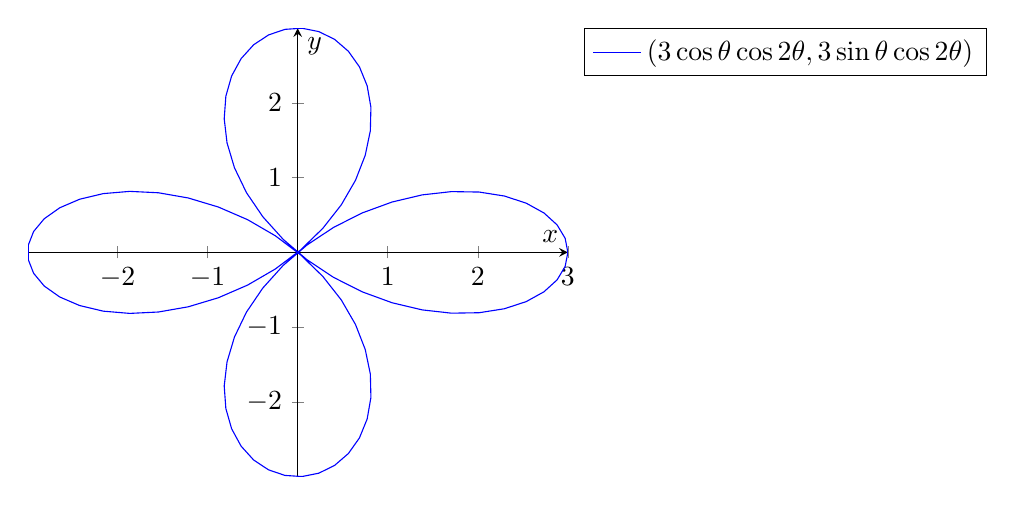
\begin{tikzpicture}
			\begin{axis}[
					axis lines = center,
					xlabel = $x$,
					ylabel = $y$,
					legend pos=outer north east
				]
				\addplot [
					domain=0:2*pi,
					samples=100,
					color=blue,
				]
				({3*cos(deg(x))*cos(deg(2*x)},
				{3*sin(deg(x))*cos(deg(2*x))});
				\addlegendentry{$(3\cos\theta\cos2\theta, 3\sin\theta\cos2\theta)$}
			\end{axis}
		\end{tikzpicture}
		We can find the area of the fan by dividing it into 8 even segments. To find the area of one segment we can find the area bounded by the curve and the $y$-axis where $x,y\geq0$
		\begin{align*}
			  & y=3\sin\theta\cos2\theta \implies \mathrm{d}y = (-6\cos\theta\sin2\theta-3\cos\theta\sin\theta)\,\mathrm{d}\theta         \\
			  & \textrm{Area} = 8\int_{\pi/4}^0 (3\cos\theta\cos2\theta)(-6\cos\theta\sin2\theta-3\cos\theta\sin\theta)\,\mathrm{d}\theta \\
			  & = 14.1\textrm{units}^2 \quad \textrm{(From G.C.)}
		\end{align*}
	\end{answer}
	\1 Find the exact volume of region $R$ rotated through 2$\pi$ radians about the $x$-axis, where $R$ is the region enclosed by $y=\dfrac{1-x}{\sqrt{x}}$, the line $x=2$ and the $x$-axis. \hfill[4]
	\begin{answer}
		\begin{tikzpicture}
			\begin{axis}[
					axis lines = center,
					xlabel = $x$,
					ylabel = $y$,
					% xtick={0,pi/2,pi,3*pi/2,2*pi},
					% xticklabels={$0$, $\frac{\pi}{2}$,$\pi$,$\frac{3}{2}\pi$,$2\pi$},
					legend pos=outer north east
				]
				\addplot [
					domain=-0.5:2.5,
					samples=100,
					color=blue,
				]
				{(1-x)/sqrt(x)};
				\addlegendentry{$\frac{1-x}{\sqrt{x}}$}
				\addplot [
					domain=-1:8,
					samples=100,
					color=red,
				]
				({2},
				{x});
				\addlegendentry{$x=2$}

			\end{axis}
		\end{tikzpicture}
		\begin{align*}
			\textrm{Volume} = \int^2_1 \pi(\frac{1-x}{\sqrt{x}})^2\,\mathrm{d}x & = \pi \int^2_1\frac{1-2x+x^2}{x}\,\mathrm{d}x                    \\
			                                                                    & = \pi \int^2_1 \frac{1}{x}-2+x\,\mathrm{d}x                      \\
			                                                                    & = \pi [\ln|x|-2+x]^2_1 = \pi(\ln2-\frac{1}{2})\;\textrm{units}^3
		\end{align*}
	\end{answer}

	\1 The curve $C$ has the equation $y=|x\mathrm{e}^x|$.
	\2 Sketch the curve $C$.\hfill[2]
	\begin{answer}
		\begin{tikzpicture}
			\begin{axis}[
					axis lines = center,
					xlabel = $x$,
					ylabel = $y$,
					legend pos=outer north east
				]
				\addplot [
					domain=-2:2,
					samples=100,
					color=blue,
				]
				{abs(x*e^x)};
				\addlegendentry{$|x\mathrm{e}^x|^2$}

			\end{axis}
		\end{tikzpicture}
	\end{answer}
	\2 Find the volume of region $S$ rotated through 2$\pi$ radians about the $x$-axis, where $S$ is the region enclosed by $C$, the lines $x=-1$ and $x=1$, and the $x$-axis.\hfill[4]
	\begin{answer}
		Integrating Repeatedly by Parts:
		\begin{align*}
			\textrm{Volume} = \pi\int^1_{-1} |x\mathrm{e}^x|^2\,\mathrm{d}x & = \pi \int^1_{-1} x^2\mathrm{e}^{2x}\,\mathrm{d}x                                                                                 \\
			                                                                & = \pi [\frac{1}{2}x^2\mathrm{e}^{2x}]^1_{-1} - \pi\int^1_{-1} x\mathrm{e}^{2x}\,\mathrm{d}x                                       \\
			                                                                & = \pi [\frac{1}{2}x^2\mathrm{e}^{2x}-\frac{1}{2}x\mathrm{e}^{2x}]^1_{-1} + \pi\int^1_{-1} \frac{1}{2}\mathrm{e}^{2x}\,\mathrm{d}x \\
			                                                                & = \pi [\frac{1}{2}x^2\mathrm{e}^{2x}-\frac{1}{2}x\mathrm{e}^{2x}+\frac{1}{4}\mathrm{e}^{2x}]^1_{-1}                               \\
			                                                                & = \pi(\frac{\mathrm{e}^2}{4}-\frac{5\mathrm{e}^{-2}}{4})\;\textrm{units}^3
		\end{align*}
	\end{answer}

	\1 The curve $C$ has the equation $\mathrm{e}^{\frac{1}{2}x-1}$.
	\2 Find the equation of $L$, where $L$ is the tangent to the curve $C$ at $x=4$.\hfill[2]
	\begin{answer}
		First we differentiate $C$ to get the gradient of the tangent.
		\begin{align*}
			         & {\frac{\mathrm{d}}{\mathrm{d}x}}(\mathrm{e}^{\frac{1}{2}x-1}) = \frac{\mathrm{e}^{\frac{x}{2}-1}}{2} \\
			         & \textrm{At} \quad x=4, y=\mathrm{e} \quad \textrm{and the gradient,} \quad m=\frac{1}{2}\mathrm{e}   \\
			         & L: y-\mathrm{e} = \frac{1}{2}\mathrm{e}(x-4)                                                         \\
			\implies & y=\frac{1}{2}\mathrm{e}x - \mathrm{e}
		\end{align*}
	\end{answer}
	\2 Find the region enclosed by $C$, $L$, and the axes.\hfill[3]
	\begin{answer}
		\begin{tikzpicture}
			\begin{axis}[
					axis lines = center,
					xlabel = $x$,
					ylabel = $y$,
					% xtick={0,pi/2,pi,3*pi/2,2*pi},
					% xticklabels={$0$, $\frac{\pi}{2}$,$\pi$,$\frac{3}{2}\pi$,$2\pi$},
					legend pos=outer north east
				]
				\addplot [
					domain=-0.5:6,
					samples=100,
					color=blue,
				]
				{e^(0.5*x-1)};
				\addlegendentry{$\mathrm{e}^{\frac{1}{2}x-1}$}
				\addplot [
					domain=-0.5:6,
					samples=100,
					color=red,
				]
				{0.5*e*x-e};
				\addlegendentry{$\frac{1}{2}\mathrm{e}x - \mathrm{e}$}

			\end{axis}
		\end{tikzpicture}
		To find the area of the region, we find the area bounded by $C$ and the $x$-axis from $(0,4)$ and then subtract the area of the triangle bounded by $L$ and the $x$-axis from $(2,4)$
		\begin{align*}
			\textrm{Area} = \int_0^4 \mathrm{e}^{\frac{1}{2}x-1}\,\mathrm{d}x - \frac{1}{2} \times 2 \times \mathrm{e} = [2\mathrm{e}^{\frac{1}{2}x-1}]_0^4 - \mathrm{e} = [\mathrm{e}-\frac{2}{\mathrm{e}}]\;\textrm{units}^2
		\end{align*}
	\end{answer}
	\2 Find the volume of the above-mentioned region when it is rotated by 2$\pi$ radians about the $y$-axis.\hfill[3]
	\begin{answer}
		To find the Volume of the region, we will take the volume of the of the region enclosed by $L$ and the $y$-axis from $(0,\mathrm{e})$ and subtract from it the volume of the region enclosed by $C$ and the $y$-axis from $(\dfrac{1}{e},\mathrm{e})$
		\begin{align*}
			\textrm{Volume} = \pi [\int_0^e (\frac{2y+2e}{e})^2 \,\mathrm{d}y - \int_0^e (2\ln{y} +2)^2 \,\mathrm{d}y] = 20.6\;\textrm{units}^3
		\end{align*}
	\end{answer}
	\1 A ball partially submerged in a beaker of water can be expressed as the following graph from the side view, where the ball is a circle and the water surface is the $x$-axis.
	\begin{figure}[h]
		\centering
		\includegraphics[width=0.4\textwidth]{integration_ball}
		\caption{Partially Submerged Ball}
	\end{figure}
	Given that the centre of the ball is at $(0,2)$ and that the radius of the ball is 4 units, show that the volume of the ball submerged in water is equal to $\frac{40}{3}\pi\;\textrm{units}^3$. \hfill[7]
	\begin{answer}
		\begin{tikzpicture}
			\begin{axis}[
					axis lines = center,
					xmin=-5, xmax=5, ymin=-3, ymax=7,
					axis equal,
					xlabel = $x$,
					ylabel = $y$,
					yticklabels={,,},
					xticklabels={,,},
				]
				\draw (axis cs: 0, 2) circle [name path=A, radius=400];
				\addplot[black, mark=*, only marks] coordinates {(0,2)};
				\node[label={180:{$(0,2)$}},circle,fill,inner sep=2pt] at (axis cs:0,2) {};

			\end{axis}
		\end{tikzpicture}
		\\The circle can be modelled by the equation $x^2 + (y-2)^2 = 4^2$. Thus, the axial intercepts are $(0,-2), (\pm2\sqrt{3}, 0)$. Let us only consider the right half of the circle. It has the equation $x = \sqrt{16-(y-2)^2}$ where $x\geq0$. We will rotate the region bounded by this new curve and the $y$-axis for the range $(0,-2)$ by 2$\pi$ radians to get the volume of the submerged region.
		\begin{align*}
			\textrm{Volume} & = \int^0_{-2} {\pi}\left[16-\left(y-2\right)^2\right]\,\mathrm{d}y = [16{\pi}y-\dfrac{{\pi}\left(y-2\right)^3}{3}]^0_{-2} =\frac{40}{3}\pi\;\textrm{units}^3
		\end{align*}
	\end{answer}
	\1 An architecture student is attempting to model the famous Burj Al Arab in wood (sculpting wood comes at \$1000.00/units$^3$). He approximates the shape of the building
	to the curve $C$ with equation $(y-k)^2 = r^2k(k-x)$ for $x,y\geq0$ where $k$ and $r$ are positive constants used for scaling purposes.
	\begin{figure}[h]
		\centering
		\includegraphics[width=0.3\textwidth]{integration_hotel}
		\caption{Burj Al Arab, taken from Wikipedia}
	\end{figure}

	\2 Given that the wooden model is formed by rotating the region enclosed by $C$ and the axes $\dfrac{\pi}{4}$ radians around the $y$-axis, calculate the volume of the model in terms of $k$ and $r$.\hfill[6]
	\begin{answer}
		\color{black}
		\begin{tikzpicture}
			\begin{axis}[
					axis lines = center,
					xmin = 0, xmax=5, ymin=0, ymax=5.3,
					xlabel = $x$,
					ylabel = $y$,
					yticklabels={,,},
					xticklabels={,,},
					legend pos=outer north east
				]
				\addplot [
					domain=-2:2,
					samples=100,
					color=blue,
				]
				({-2*x^2+1.5},{4*x+1.5});
				\addlegendentry{$(y-k)^2 = r^2k(k-x)$}

				% Add a mark and then label the coordinates %
				\addplot[black, mark=*, only marks] coordinates {(1.21875,0)}; % This makes the dot %
				\node[label={180:{$(k,0)$}}] at (axis cs:1.21875,0.3) {}; % This is the coordinates %

				\addplot[black, mark=*, only marks] coordinates {(0,4.964101615)}; % This makes the dot %
				\node[label={180:{$(0,rk+k)$}}] at (axis cs:1.8,4.8) {}; % This is the words %

			\end{axis}
		\end{tikzpicture}
		\color{blue}
		\\First, we transpose $C$ down by $k$-units, effectively replacing $y-k$ with $y$. \\
		\color{black}
		\begin{tikzpicture}
			\begin{axis}[
					axis lines = center,
					xmin = 0, xmax=5, ymin=-1.6, ymax=3.8,
					xlabel = $x$,
					ylabel = $y$,
					yticklabels={,,},
					xticklabels={,,},
					legend pos=outer north east
				]
				\addplot [
					domain=-2:2,
					samples=100,
					color=red,
				]
				({-2*x^2+1.5},{4*x});
				\addlegendentry{$y^2 = r^2k(k-x)$}

				\addplot[black, mark=*, only marks] coordinates {(0,3.564101615)};
				\node[label={180:{$(0,rk)$}}] at (axis cs:1.3,3.3) {};

				\addplot[black, mark=*, only marks] coordinates {(0,-1.5)};
				\node[label={180:{$y=-k$}}] at (axis cs:1.3,-1.2) {};

				\addplot[mark=none, black, ultra thick,dotted] coordinates {(0,-1.5) (1.21875,-1.5)};

			\end{axis}
		\end{tikzpicture}
		\color{blue}
		\\Following which, we find the volume of the region bounded by $C$ and the $y$-axis by integrating with respect to $y$ from $(-k,rk)$. Since we are rotating the region by only $\dfrac{\pi}{4}$ radians, we multiply the integral by only $\frac{\pi}{8}$ instead of $\pi$
		\begin{align*}
			\textrm{Volume} & = \frac{\pi}{8}\int_{-k}^{rk}\left(k-\dfrac{y^2}{r^2k}\right)^2\,\mathrm{d}y                   \\
			                & = \frac{\pi}{8}\int_{-k}^{rk}\left(\dfrac{y^4}{k^2r^4}-\dfrac{2y^2}{r^2}+k^2\right)\mathrm{d}y \\
			                & = \frac{\pi}{8}[\frac{y^5}{5k^2r^4}-\frac{2y^3}{3r^2}+k^2y]_{-k}^{rk}                          \\
			                & = \dfrac{{\pi}k^3\left(8r^5+15r^4-10r^2+3\right)}{120r^4}
		\end{align*}
	\end{answer}
	\2 Calculate the amount of money spent on wood by the architecture student to construct the model if $k=1,r=\frac{3}{2}$.\hfill[3]
	\begin{answer}
		\begin{align*}
			\textrm{Cost} & = \dfrac{{\pi}\cdot1^3\left[8(1.5)^5+15(1.5)^4-10(1.5)^2+3\right]}{120(1.5)^4}\times \$1000 \\
			              & = \frac{125\pi}{648}\times \$1000                                                           \\
			              & = \$606.02 \quad \textrm{(Nearest cent)}
		\end{align*}
	\end{answer}
\end{outline}
\end{document}
